\documentclass[11pt]{article}
\usepackage[a4paper,margin=2.4cm]{geometry}
\usepackage[T1]{fontenc}
\usepackage{lmodern}
\usepackage{microtype}
\usepackage{amsmath}
\usepackage{booktabs}
\usepackage{graphicx}
\usepackage{xcolor}
\usepackage[hidelinks]{hyperref}
\usepackage[numbers,sort&compress]{natbib}
\usepackage{caption}
\usepackage[section]{placeins}
\captionsetup{font=small,labelfont=bf}
\setlength{\parskip}{0.35em}

% Written by make_numbers.py from the result files; do not edit.
\newcommand{\beliefSteady}{87.1\%}
\newcommand{\beliefSwitch}{50}
\newcommand{\clAround}{70\%}
\newcommand{\clAroundFourFalse}{1.1}
\newcommand{\clAroundThree}{89\%}
\newcommand{\clAroundThreeFalse}{3.3}
\newcommand{\clBrows}{35\%}
\newcommand{\clClenchBursts}{1,447}
\newcommand{\clHeadband}{52\%}
\newcommand{\clListen}{5.7}
\newcommand{\clListenDouble}{0.11}
\newcommand{\clListenHours}{18}
\newcommand{\clListenOthers}{5.6}
\newcommand{\clScalp}{99\%}
\newcommand{\clSwallow}{51\%}
\newcommand{\clSwallowAuc}{0.62}
\newcommand{\clSwallowBest}{0.66}
\newcommand{\clSwallowKeep}{1\%}
\newcommand{\clSwallowN}{104}
\newcommand{\clTongue}{1.3\%}
\newcommand{\earAroundLin}{56.9\%}
\newcommand{\earAroundLinFive}{64.4\%}
\newcommand{\earAroundNn}{61.0\%}
\newcommand{\earAroundNnFive}{71.1\%}
\newcommand{\earBothLin}{49.3\%}
\newcommand{\earBothLinFive}{43.3\%}
\newcommand{\earBothNn}{59.0\%}
\newcommand{\earBothNnFive}{60.0\%}
\newcommand{\earInLin}{48.6\%}
\newcommand{\earInLinFive}{42.2\%}
\newcommand{\earInNn}{48.3\%}
\newcommand{\earInNnFive}{45.6\%}
\newcommand{\earScalpLin}{74.1\%}
\newcommand{\earScalpLinFive}{95.6\%}
\newcommand{\earScalpNn}{80.9\%}
\newcommand{\earScalpNnFive}{95.6\%}
\newcommand{\gateBlanked}{6\%}
\newcommand{\gateOffFive}{91.0\%}
\newcommand{\gateOffSixty}{78.9\%}
\newcommand{\gateOffTen}{64.1\%}
\newcommand{\gateOnFive}{92.1\%}
\newcommand{\gateOnSixty}{79.2\%}
\newcommand{\gateOnTen}{63.9\%}
\newcommand{\heldContentCtl}{48.3\%}
\newcommand{\heldContentFiveMin}{87.5\%}
\newcommand{\heldContentSixty}{75.9\%}
\newcommand{\heldContentTen}{61.4\%}
\newcommand{\heldStandardCtl}{48.4\%}
\newcommand{\heldStandardFiveMin}{91.2\%}
\newcommand{\heldStandardSixty}{75.6\%}
\newcommand{\heldStandardTen}{61.7\%}
\newcommand{\heldStudyCtl}{47.6\%}
\newcommand{\heldStudyFiveMin}{86.1\%}
\newcommand{\heldStudySixty}{72.1\%}
\newcommand{\heldStudyTen}{60.0\%}
\newcommand{\holdCovertEeg}{88\%}
\newcommand{\holdCovertFace}{13\%}
\newcommand{\holdCovertFused}{43\%}
\newcommand{\holdCovertFusedDwell}{51\%}
\newcommand{\holdCovertFusedKOne}{72\%}
\newcommand{\holdCovertHeadDwell}{13\%}
\newcommand{\holdCovertHold}{16\%}
\newcommand{\holdEeg}{87.1\%}
\newcommand{\holdFace}{75.5\%}
\newcommand{\holdFused}{88.6\%}
\newcommand{\holdFusedDwell}{92.0\%}
\newcommand{\holdFusedKOne}{91.6\%}
\newcommand{\holdHeadDwell}{86.8\%}
\newcommand{\holdHold}{84.2\%}
\newcommand{\holdNobodyFusedDwell}{95.8\%}
\newcommand{\holdNobodyHeadDwell}{99.5\%}
\newcommand{\holdOtherFused}{81.7\%}
\newcommand{\holdOtherFusedDwell}{87.5\%}
\newcommand{\holdOtherHeadDwell}{76.6\%}
\newcommand{\holdSwitchTook}{20}
\newcommand{\holdSwitchTookKOne}{10}
\newcommand{\hwArtifactsBase}{78.1\%}
\newcommand{\hwArtifactsBreaks}{2}
\newcommand{\hwArtifactsHolds}{1}
\newcommand{\hwArtifactsTen}{63.5\%}
\newcommand{\hwArtifactsTwo}{72.7\%}
\newcommand{\hwArtifactsWorst}{60.6\%}
\newcommand{\hwBurstBase}{78.1\%}
\newcommand{\hwBurstBreaks}{20\%}
\newcommand{\hwBurstHolds}{none}
\newcommand{\hwBurstWorst}{73.4\%}
\newcommand{\hwCrosstalkBase}{78.1\%}
\newcommand{\hwCrosstalkBreaks}{beyond the range}
\newcommand{\hwCrosstalkHolds}{70\%}
\newcommand{\hwCrosstalkWorst}{77.2\%}
\newcommand{\hwEnvlagBase}{78.1\%}
\newcommand{\hwEnvlagBreaks}{50}
\newcommand{\hwEnvlagEarly}{76.8\%}
\newcommand{\hwEnvlagHolds}{none}
\newcommand{\hwEnvlagLate}{75.7\%}
\newcommand{\hwEnvlagWorst}{55.7\%}
\newcommand{\hwGatecClean}{79.8\%}
\newcommand{\hwGatecTen}{71.5\%}
\newcommand{\hwGatecTwo}{77.2\%}
\newcommand{\hwGatedBase}{78.7\%}
\newcommand{\hwGatedBreaks}{5}
\newcommand{\hwGatedClean}{78.7\%}
\newcommand{\hwGatedHolds}{none}
\newcommand{\hwGatedTen}{70.1\%}
\newcommand{\hwGatedTwo}{77.8\%}
\newcommand{\hwGatedWorst}{62.1\%}
\newcommand{\hwLossBase}{78.1\%}
\newcommand{\hwLossBreaks}{40\%}
\newcommand{\hwLossHolds}{10\%}
\newcommand{\hwLossWorst}{73.8\%}
\newcommand{\hwLsbBase}{78.1\%}
\newcommand{\hwLsbBreaks}{20}
\newcommand{\hwLsbHolds}{10}
\newcommand{\hwLsbWorst}{72.6\%}
\newcommand{\hwMainsBase}{78.1\%}
\newcommand{\hwMainsBreaks}{50000}
\newcommand{\hwMainsHolds}{10000}
\newcommand{\hwMainsWorst}{72.9\%}
\newcommand{\hwNets}{2}
\newcommand{\hwNoiseBase}{78.1\%}
\newcommand{\hwNoiseBreaks}{1600}
\newcommand{\hwNoiseHolds}{100}
\newcommand{\hwNoiseWorst}{60.2\%}
\newcommand{\hwPinkBase}{78.1\%}
\newcommand{\hwPinkBreaks}{2}
\newcommand{\hwPinkHolds}{0.5}
\newcommand{\hwPinkWorst}{57.2\%}
\newcommand{\hwRateBase}{78.1\%}
\newcommand{\hwRateBreaks}{beyond the range}
\newcommand{\hwRateHolds}{100}
\newcommand{\hwRateWorst}{78.1\%}
\newcommand{\hwSkewBase}{78.1\%}
\newcommand{\hwSkewBreaks}{80}
\newcommand{\hwSkewHolds}{20}
\newcommand{\hwSkewWorst}{64.3\%}
\newcommand{\linFiveMin}{85.2\%}
\newcommand{\linMesd}{120}
\newcommand{\linPast}{25}
\newcommand{\linSixty}{68.1\%}
\newcommand{\linTen}{58.0\%}
\newcommand{\linTwo}{54.2\%}
\newcommand{\nnCtlSixty}{49.0\%}
\newcommand{\nnCtlTen}{50.3\%}
\newcommand{\nnFiveMin}{91.0\%}
\newcommand{\nnMesd}{57}
\newcommand{\nnPast}{30}
\newcommand{\nnSixty}{78.9\%}
\newcommand{\nnSplits}{79.4\%, 78.1\%, 79.2\%}
\newcommand{\nnTen}{64.1\%}
\newcommand{\nnTenMin}{96.9\%}
\newcommand{\nnTwo}{56.6\%}
\newcommand{\onsetFiveTen}{90.7\%}
\newcommand{\onsetFiveThirty}{91.7\%}
\newcommand{\onsetFiveZero}{91.2\%}
\newcommand{\scaleLinAll}{68.1\%}
\newcommand{\scaleLinFifteen}{67.6\%}
\newcommand{\scaleLinTwo}{61.1\%}
\newcommand{\scaleNnAll}{76.1\%}
\newcommand{\scaleNnFifteen}{73.2\%}
\newcommand{\scaleNnFive}{67.5\%}
\newcommand{\scaleNnTen}{70.7\%}
\newcommand{\scaleNnTwenty}{75.2\%}
\newcommand{\spliceFollowed}{75\%}
\newcommand{\spliceMedian}{43}
\newcommand{\spliceSteady}{74.9\%}
\providecommand{\missing}{??}


\title{Attention decoding for true wireless earbuds:\\ calibration free, held out by person, story and study,\\ and what it asks of the hardware}
\author{Artun Balta\\ \small Signalive}
\date{\small Preprint, November 2026}

\begin{document}
\maketitle

\begin{abstract}
Auditory attention decoding could let earbuds know which voice their wearer follows. But an earbud cannot be calibrated for each person, its two sides share no electrical reference, it must be causal, and it must work for people and speech it never met. Under those four conditions throughout, on public recordings, a learned decoder over four electrodes around each ear names the followed story in \nnSixty{} of one minute decisions and \nnFiveMin{} of five minute ones for 36 people it never saw (a linear decoder: \linSixty{}; chance: 50\%), keeps its accuracy on story content and on a source study it never trained on, and falls to chance when the speech is moved out of step. On 15 other people recorded in the ear, around it and on the scalp at the same moments, dry contacts in the ear canal decode at chance (\earInNn{}) while contacts around the ear reach \earAroundNn{}: an earbud's contacts must reach outside the canal. Replaying the real decisions under a head that looks away shows where the EEG adds to head direction, which is when the listener looks at someone other than the person followed and when attention moves while the head stays, and that the head should be weighed less than a hand set default. Degrading the raw recordings sets the electronics' tolerances. A jaw clench detector, run unchanged on four public datasets, catches \clAround{} of cued clenches around the ear, and a double clench fires by itself \clListenDouble{} times an hour in quiet listening against \clListenOthers{} for singles and holds, which makes the double clench the command that must not fire by accident.

\end{abstract}

\section{Introduction}

A listener in a group can follow one voice among several, and the brain's response follows the envelope of the voice that is followed more closely than the envelope of the others \cite{geirnaert2021}. Auditory attention decoding (AAD) reads that difference from EEG: a decoder relates the EEG to each candidate talker's speech envelope and names the talker it matches best. Electrodes around and inside the ear make the measurement wearable \cite{mirkovic2016,kidmose2013,geirnaert2025}, which raises the question of what an earbud could do with it.

A consumer earbud sets four conditions that laboratory AAD usually relaxes. It cannot ask each wearer to calibrate the decoder on labelled data. Two true wireless earbuds share no electrical reference, so each ear must be referenced to itself. Everything must be causal, with a bounded look ahead. And its claims must hold for people, speech and recording conditions the decoder never saw, because cross validation that shares any of them can flatter a decoder: a model trained on the same stories as the test listeners may learn the stories rather than the tracking \cite{puffay2023,detaillez2020}, and spatial decoders can follow the block design rather than attention \cite{rotaru2024,yan2025}.

This paper reports what public recordings say about such an earbud, under those four conditions throughout.
\begin{itemize}
\item A learned decoder for eight electrodes around the ears, four per ear and each ear referenced to itself, trained on other people only and evaluated causally. It is tested on held out people, on held out story content and on a held out source study, each with an out of step control.
\item A decision weight fitted by maximum likelihood and a two state hidden Markov belief, which turn weak ten second decisions into a stable estimate, timed on real EEG cut together from listeners who followed opposite stories.
\item A replay of those decisions under a head that looks away, which says when the EEG adds anything to head direction and how much the head should weigh against it.
\item A comparison of dry in-ear, wet around-ear and scalp electrodes recorded at the same moments from the same people, with the same calibration free protocol and each ear self referenced.
\item The tolerances the decoder implies for the earbud's electronics, measured by degrading the raw recordings: noise, resolution, sampling rate, clock offset between the two earbuds, lost packets, movement artifacts, mains interference and the timing of the speech envelopes.
\item A jaw clench command detector, the earbud's silent input, run unchanged on four public datasets of real clenches and of the movements that resemble them.
\end{itemize}
The code that runs on the phone is the code evaluated here: a TypeScript port of every step, checked against the reference implementation to within $10^{-9}$.

\section{Data}

\paragraph{Attention around the ear.} OpenNeuro ds004015 \cite{ds004015,holtze2022} pools 36 participants from two studies \cite{jaeger2020,holtze2021} who listened to two audiobooks at once, one from the left and one from the right, and followed one side throughout. Eighteen cEEGrid electrodes around the two ears were recorded at 500~Hz against an electrode behind the right ear. Each person has three equally loud 10 minute blocks selected by the dataset (the test set here) and two more: two equally loud blocks for the first study's participants, and two blocks in which the followed story was louder for the second's, which only ever train a model here. The dataset ships each story's speech envelope at 64~Hz, not the audio. Every participant heard the same story parts in the same blocks, with story 1 always on the left.

\paragraph{In the ear and around it.} Ear-SAAD \cite{earsaad,geirnaert2025} has 15 participants, each with six 10 minute trials of two competing Danish lectures at $\pm60^\circ$, attending the left talker in some trials and the right in others. Recorded at once at 1000~Hz: 29 scalp channels, 9 and 10 wet electrodes around the left and right ear, and 6 dry electrodes in each ear canal and concha. Its description file gives the license as CC BY-NC-SA 4.0; it is used for research and only results are reported.

\paragraph{Clenches and what resembles them.} Park et al.\ \cite{park2023ear}: 15 participants, 18 electrodes around the ears at 250~Hz, ten cued 3~s clenches each, and recordings of blinking, eye movements, rest with eyes open and closed, and heartbeat. Lee and Ahn \cite{leeahn2026}: a consumer headband (Muse 2) with one electrode behind each ear at 256~Hz, 20 cued clenches per person, blinks and head movements. PhysioMotion \cite{physiomotion}: 59 scalp channels at 1000~Hz with swallowing, tongue movement as in speech, eyebrow raises, head turns and nods, blinks and cued molar clenching, each marked by two annotators; 12 of its 30 participants are used. And the 18 hours of quiet listening in ds004015 at 500~Hz, in which no one was asked to clench.

\section{Methods}

\subsection{The signal chain}
Each electrode passes a causal second order Butterworth band pass from 1 to 9~Hz at its recording rate and is resampled to 64~Hz by linear interpolation; the earbud runs the same steps, sample by sample. For two separate earbuds the four electrodes of each ear are referenced to their own average (the \emph{wireless} montage); the electrodes are the four per ear that a greedy search ranked best on the group. Each derived channel is scaled by its spread over the person's first two minutes, unlabelled. Each envelope is band passed the same way and scaled by its own running spread (an exponential average over 30~s). No step reads a sample from more than 0.47~s ahead of the moment it outputs.

\subsection{Decoders}
\label{sec:decoders}
\paragraph{Linear.} A backward model rebuilds the followed envelope from every channel at lags of 0 to 484~ms by ridge regression, its strength chosen by inner cross validation; a window's verdict is the story whose envelope correlates best with the rebuilt one.
\paragraph{Learned.} Two small convolutional networks map the EEG and each envelope to 12 dimensional embeddings: a $1\times1$ mix to 24 channels, then dilated convolutions with GELU and dropout, then a $1\times1$ mix to the embedding, about 16,000 weights each; the envelope network also sees half a second of its story before each EEG sample. Training takes random 5~s crops and asks, by cross entropy over the two stories, that the followed story's embedding move with the EEG's: the mean over time of their per sample product, each centred and scaled by its mean norm within the window. A window of any length is judged by the same score over that window alone, so one model serves every decision length.
\paragraph{Choosing the settings.} Variants of the data, network and training were compared by the mean validation log loss of their ten second decisions, on the five validation people of each fold only, with the rule fixed before any run; test numbers were recorded but never used to choose.

\subsection{Evaluation}
\paragraph{People.} Six folds of six test people; of the other thirty, five stop training and the rest train it. Each person's accuracy is averaged over three random splits, each with its own models. A one minute decision is significant for one person at 66.7\% over 30 minutes (one sided binomial, 5\%).
\paragraph{Story content.} Every test block is scored by models trained on no block of the same story parts, from anyone: for each part, the models of a fold are retrained without it.
\paragraph{Study.} Models trained on one source study are tested on the other, in both directions.
\paragraph{Out of step.} The same models score the same windows with both envelopes rotated 97~s against the EEG: the same voices, out of step. A decoder that tracks speech falls to chance; one that recognised the voices and read something else from the EEG would not.
\paragraph{Switch time.} Accuracy over window length becomes a minimal expected switch duration (MESD) \cite{geirnaert2019mesd}; and the belief below is timed on real switches made by cutting together, at random times, the EEG of a held out listener who followed one story with that of another, from the same fold, who followed the other over the same blocks.

\subsection{From decisions to a belief}
A ten second decision moves the phone's estimate by $\exp(w\,m)$, $m$ being the margin of the winning story's score; $w$ is fitted by maximum likelihood on held out decisions. A two state hidden Markov model filters these decisions forward, with a chance $h$ per decision that attention moved; $h$ trades steadiness against speed.

\subsection{Holding the talker}
Each held out person's ten second decisions, in order, are replayed under a simulated head. Every ten second step the head faces the followed talker, nobody, or the other talker (at $\pm60^\circ$, with 10 or 20 degrees of jitter), by a Markov chain that keeps the current state with probability $e^{-10/20}$ per step and otherwise draws a new one from set shares; the share of time looking away and how it divides between nobody and the other talker are swept. Six ways of choosing the voice brought forward are compared: the talker faced (within $30^\circ$); the same, holding the last talker faced while facing nobody; the same, changing only after 20~s on a new talker; the belief alone; the phone's fusion of head prior and belief at its default weight $\kappa=2$; and the fusion at $\kappa=1$. Each is scored on blocks where attention stays (the share of steps from the second minute on with the followed voice forward), on blocks where attention and head switch together at a random moment (the decisions after it flipped, as in the belief's own test, and the time until the new voice comes forward), and on blocks where attention switches but the head goes on as before.

\subsection{Hardware tolerances}
The raw 500~Hz recordings of each held out person are degraded as a cheaper or harsher earbud would degrade them, then pass the whole causal chain and the models that never saw that person: white and $1/f$ noise at every electrode, quantisation to a given step, a lower sampling rate behind an anti alias filter, the right earbud's clock offset against the left, lost 20~ms and 200~ms frames with the last sample held, movement artifacts (200~$\mu$V Hann bumps of 0.2 to 1~s on every electrode with unequal gains), 50~Hz mains common to every electrode with 1\% imbalance, and speech envelopes late or early against the EEG.

\subsection{The clench detector}
The detector runs on the phone. Per ear it averages the 30 to 120~Hz power of that ear's electrodes into a 50~ms RMS, compared with an adaptive floor; a burst needs both ears above $k$ times their floor ($k=4$) for 40~ms. Bursts become a single, a double (two bursts of at most 450~ms within 450~ms) or a hold (over 700~ms); four bursts within 3~s are chewing, which silences it for 2~s and withdraws the gestures it reported since the first of those bursts. It is run unchanged, sample by sample, on every recording in Section~2.

\section{Results}
\subsection{Decoding, held out by person}
\label{sec:decoding}

\begin{figure}[t]
\centering
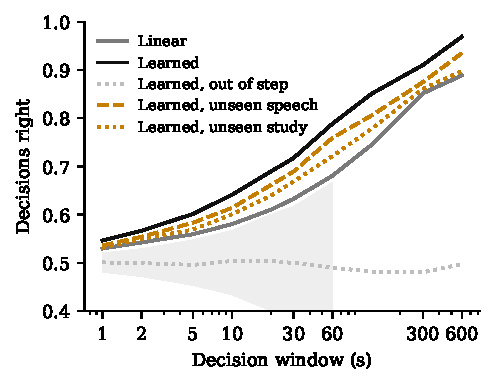
\includegraphics[width=\linewidth]{fig_windows.pdf}
\caption{Share of decisions that name the followed story against the length of EEG a decision may use, for 36 people decoded by models that never saw them: four electrodes per ear, each ear referenced to itself, no calibration. Shaded: where one person's 30 minutes cannot be told from chance (one sided binomial, 5\%). Dotted grey: the learned decoder with the speech moved 97~s out of step. Amber: one learned network per fold trained without the story content tested (dashed) or without the source study tested (dotted).}
\label{fig:windows}
\end{figure}

\begin{table}[t]
\centering
\caption{Share of decisions that name the followed story, mean over 36 held out people, four electrodes per ear, each ear referenced to itself, no calibration. Chance is 50\%. MESD: median minimal expected switch duration. Past bar: people whose one minute decisions over 30 minutes beat chance for one person (66.7\%).}
\label{tab:main}
\begin{tabular}{lrrrrrr}
\toprule
Decoder & 2~s & 10~s & 60~s & 5~min & MESD & Past bar \\
\midrule
Linear & \linTwo & \linTen & \linSixty & \linFiveMin & \linMesd~s & \linPast{} of 36 \\
Learned & \nnTwo & \nnTen & \nnSixty & \nnFiveMin & \nnMesd~s & \nnPast{} of 36 \\
Learned, out of step & & \nnCtlTen & \nnCtlSixty & & & \\
\bottomrule
\end{tabular}
\end{table}

Of the thirteen training variants compared on validation people alone, the lowest validation log loss of ten second decisions went to the base architecture trained on all five blocks per person with a learning rate of $10^{-3}$ (0.6356; a wider receptive field scored 0.6357, inside the tie margin that goes to the simpler variant; every other variant 0.6378 or more). That variant, as an ensemble of five networks per fold, names the followed story in \nnSixty{} of one minute decisions and \nnFiveMin{} of five minute ones, against \linSixty{} and \linFiveMin{} for the linear decoder (Table~\ref{tab:main}, Figure~\ref{fig:windows}), and \nnTenMin{} over ten minutes. The three random splits of the people gave \nnSplits{} at one minute. Moved 97~s out of step with the EEG, the same speech scores \nnCtlSixty{}. Every story starts at its block's first sample, so the onset of the sound could in principle carry the answer in the first window: dropping the first 10 or 30~s of every block, EEG and stories alike, left five minute accuracy at \onsetFiveTen{} and \onsetFiveThirty{} against \onsetFiveZero{} (split 7).

\subsection{Held out by story and by study}
\label{sec:heldout}

\begin{table}[t]
\centering
\caption{One network per fold (split 7), the settings of the search: what is held out besides the test people.}
\label{tab:heldout}
\begin{tabular}{lrrrr}
\toprule
Also held out & 10~s & 60~s & 5~min & Out of step, 60~s \\
\midrule
Nothing & \heldStandardTen & \heldStandardSixty & \heldStandardFiveMin & \heldStandardCtl \\
The story content tested & \heldContentTen & \heldContentSixty & \heldContentFiveMin & \heldContentCtl \\
The source study & \heldStudyTen & \heldStudySixty & \heldStudyFiveMin & \heldStudyCtl \\
\bottomrule
\end{tabular}
\end{table}

Trained without any block of the story content it was tested on, the network kept its one minute accuracy (\heldContentSixty{} against \heldStandardSixty{}) and lost a few points at five minutes; trained on one source study and tested on the other, it kept \heldStudySixty{} (Table~\ref{tab:heldout}).

\begin{table}[t]
\centering
\caption{Published one minute accuracies with electrodes around the ear, each under its own protocol, and this decoder. SS: trained on the person tested; SI: trained on other people only.}
\label{tab:lit}
\begin{tabular}{llr}
\toprule
Study & Electrodes, training & 60~s \\
\midrule
Mirkovic et al.\ \cite{mirkovic2016} & cEEGrid, 16, linked mastoids, SS & 69.3\% \\
Holtze et al.\ \cite{holtze2022} (this data set) & cEEGrid, 16, SS & 71.3\% \\
Geirnaert, Kappel, Kidmose \cite{geirnaert2025} & 19 around the ear, SS & 67.2\% \\
This work & 8, each ear referenced to itself, SI & \nnSixty \\
\bottomrule
\end{tabular}
\end{table}

\subsection{From decisions to a belief}
\label{sec:belief}

A ten second decision of the learned decoder is right \nnTen{} of the time. Fed into the belief with the fitted weight and a switch chance of 0.02 per decision, it favours the followed story after \beliefSteady{} of decisions from the second minute on. On EEG cut together from two held out listeners who followed opposite stories, the belief came over to the new story in a median of \spliceMedian~s, for \spliceFollowed{} of the switches it was in a position to follow, and favoured the followed story \spliceSteady{} of the time more than a minute after a cut.

\subsection{What holding the talker is worth}
\label{sec:hold}

Every held out person's ten second decisions were replayed under a head that sometimes looks away, by a Markov chain over three states per ten second step (facing the followed talker, facing nobody, facing the other talker, at $\pm60^\circ$), with a mean look of 20~s; the share of time looking away is an assumption and was swept. With a quarter of the time looking away, half of it at the other talker, the followed voice was the one brought forward in \holdFace{} of steps when the head alone chose (the talker faced), \holdHold{} when the last talker faced was held while facing nobody, and \holdHeadDwell{} when a new talker had to be faced for 20~s first. The belief alone gave \holdEeg{}; the phone's fusion of head and belief \holdFused{}; with the head weighed half as much ($\kappa=1$) \holdFusedKOne{}, following a real turn in a median \holdSwitchTookKOne~s; and with the head's weight growing over the first 40~s of facing a talker \holdFusedDwell{}, at a median \holdSwitchTook~s. Looking away only at nobody, the patient head rule alone reached \holdNobodyHeadDwell{}, and the belief added nothing; looking away only at the other talker, it reached \holdOtherHeadDwell{}, against \holdOtherFusedDwell{} with the dwell fusion. When attention moved and the head did not, only the belief followed: the new talker was forward in \holdCovertEeg{} of the last two minutes, against \holdCovertHeadDwell{} for the head rule, \holdCovertFused{} for the phone's fusion and \holdCovertFusedKOne{} with the head weighed half.

\subsection{In the ear and around it}
\label{sec:ear}

\begin{table}[t]
\centering
\caption{Ear-SAAD, 15 people, every person decoded by models trained on other people only, each ear referenced to itself (the scalp to its common average), causal, from the 10th second of each trial.}
\label{tab:ear}
\begin{tabular}{lrrr}
\toprule
Electrodes & Linear, 60~s & Learned, 60~s & Learned, 5~min \\
\midrule
In the ear, dry, 6 per ear & \earInLin & \earInNn & \earInNnFive \\
Around the ear, wet, 9 and 10 & \earAroundLin & \earAroundNn & \earAroundNnFive \\
Both together & \earBothLin & \earBothNn & \earBothNnFive \\
Scalp, 29 & \earScalpLin & \earScalpNn & \earScalpNnFive \\
\bottomrule
\end{tabular}
\end{table}

With dry contacts in the ear, neither decoder did better than chance; around the ear, the learned decoder reached \earAroundNn{} at one minute, and together the two sets did worse than around the ear alone (Table~\ref{tab:ear}). On the scalp, the same chain and decoders reached \earScalpNn{}. The out of step control stayed between 47\% and 51\% for every montage.

\subsection{How accuracy grows with the people trained on}
\label{sec:scaling}

Trained on $N$ people drawn from the other 35, the linear decoder's one minute accuracy rose from \scaleLinTwo{} with two to \scaleLinFifteen{} with fifteen and then stopped: \scaleLinAll{} with all 35. The learned decoder, a single network per fold trained on 5 to 25 of each fold's people and averaged over the three splits, reached \scaleNnFive{}, \scaleNnTen{}, \scaleNnFifteen{}, \scaleNnTwenty{} and \scaleNnAll{}, still rising when the folds ran out of people to train it on.

\subsection{What the electronics may add}
\label{sec:hardware}

\begin{figure}[t]
\centering
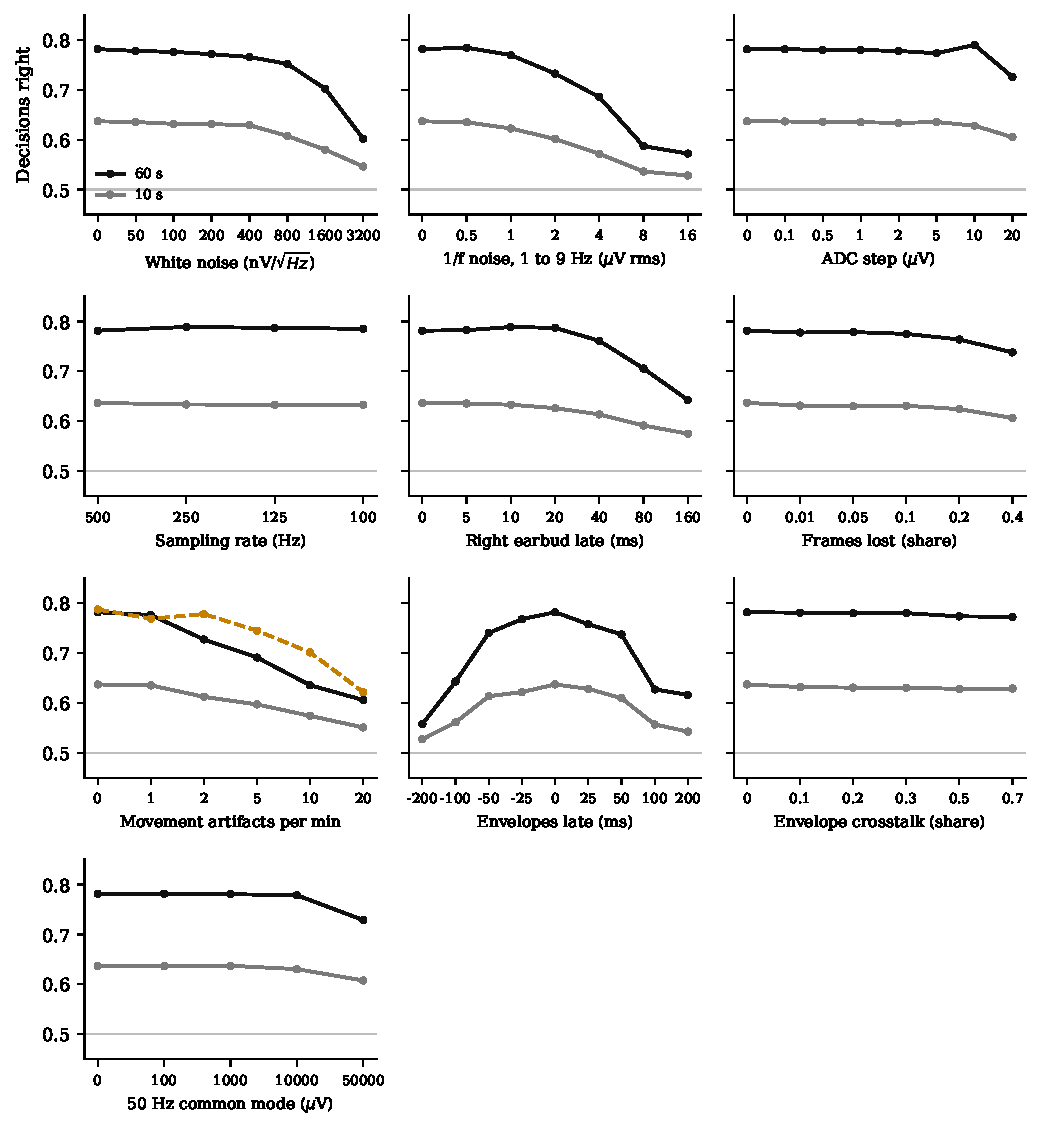
\includegraphics[width=\linewidth]{fig_hardware.pdf}
\caption{Accuracy of the final decoder (split 7, \hwNets{} networks per fold) on the raw recordings of people it never saw, degraded as an earbud's electronics might degrade them; one panel per degradation, the clean recording at its first level (at 0~ms in the envelope panel). Black: one minute decisions; grey: ten second ones; amber, dashed: one minute decisions with movement artifacts gated.}
\label{fig:hardware}
\end{figure}

Against a clean one minute accuracy of \hwNoiseBase{} with these networks (Figure~\ref{fig:hardware}), white noise added at every electrode cost less than a point up to \hwNoiseHolds{}~nV/$\sqrt{\mathrm{Hz}}$ and three points at \hwNoiseBreaks{}; 1/f noise in the decoder's band, up to \hwPinkHolds{}~$\mu$Vrms; one converter step, up to \hwLsbHolds{}~$\mu$V; and sampling, down to \hwRateHolds{}~Hz. A clock offset between the two earbuds cost nothing up to \hwSkewHolds{}~ms and three points at \hwSkewBreaks{}~ms. Frames lost one at a time cost under a point up to \hwLossHolds{} of all frames, and three points at \hwLossBreaks{}; lost in 200~ms bursts, three points at \hwBurstBreaks{}. Mains at 50~Hz, common to every electrode with 1\% imbalance, did nothing up to \hwMainsHolds{}~$\mu$V. The speech envelopes were the strictest: 25~ms late against the EEG they brought one minute accuracy to \hwEnvlagLate{}, 25~ms early to \hwEnvlagEarly{}, and three points were lost at \hwEnvlagBreaks{}~ms; the other talker mixed into each envelope, as imperfect separation would leave it, cost under a point up to \hwCrosstalkHolds{} of it.

Movement was the one degradation that cost much at a plausible rate: two 200~$\mu$V jolts a minute brought one minute accuracy to \hwArtifactsTwo{} and ten to \hwArtifactsTen{}. A gate that blanks a quarter second either side of any sample over five times its channel's spread kept \hwGatedTwo{} and \hwGatedTen{} at those rates, and on the clean recording \hwGatedClean{}: it costs nothing and belongs in the chain.


\subsection{The clench, on real recordings}
\label{sec:clench}

\begin{figure}[t]
\centering
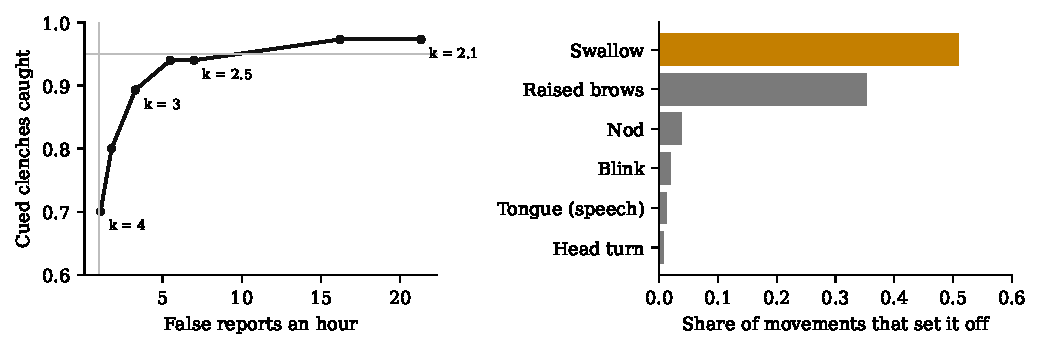
\includegraphics[width=\linewidth]{fig_clench.pdf}
\caption{The phone's clench detector, unchanged. Left: around the ear (15 people, 250~Hz), cued 3~s clenches caught against false reports an hour in blinking, eye movements, rest and heartbeat, for thresholds $k$ from 2.1 to 4 (shipped); grey lines mark the bars of 95\% caught and one false report an hour. Right: the share of each labelled movement during which it reported a gesture (12 people, temporal scalp, 1000~Hz).}
\label{fig:clench}
\end{figure}

At the shipped threshold the detector caught \clAround{} of cued clenches around the ear, \clHeadband{} on a consumer headband with one electrode behind each ear, and \clScalp{} of cued clench blocks on the temporal scalp at 1000~Hz. Around the ear the misses were concentrated: ten of fifteen people had nine or ten of their ten clenches caught, five had three or fewer, and in those five the muscle signal of the weaker ear rose only 2.4 to 3.9 times above its background during a clench, under the threshold of four. Lowering the threshold catches them and costs false reports (Figure~\ref{fig:clench}, left): \clAroundThree{} of clenches at \clAroundThreeFalse{} false an hour for $k=3$, against \clAroundFourFalse{} for $k=4$. A personal threshold set from each person's first three clenches did not reliably beat a fixed one: chosen on half the people it caught every later clench at 1.4 false an hour, and on the other half 84\% at 7.1.

Every recording without a cued clench measures false reports. In 89 minutes of rest and heartbeat around the ear there were three, in 74 minutes of blinking and eye movement none, and on the headband none at rest, six an hour while blinking and fifteen while moving the head. In \clListenHours{} hours of quiet listening (ds004015, 500~Hz, the earbud's four electrodes per ear) there were \clListen{} an hour: the median listener two, the worst 37. By labelled movement, swallowing set the detector off \clSwallow{} of the time and raised eyebrows \clBrows{}, while tongue movement as in speech did \clTongue{}, head nods and turns 0.7 to 3.8\%, blinks 1.9\% and eye movements never (Figure~\ref{fig:clench}, right).

Double clenches were the exception everywhere: \clListenDouble{} false doubles an hour in quiet listening against \clListenOthers{} singles and holds, none in the labelled movements apart from 2 of 452 tongue movements, and in every recording 20 to 50 times rarer than a false single.

Swallows could not be rejected in software. Described by what the detector could compute as it goes (the weaker ear's peak over its background, the time above half the peak, slow potentials during the event, upper against lower contacts, spectral balance and symmetry), the \clSwallowN{} labelled swallows and the \clClenchBursts{} bursts inside the cued clench blocks overlapped on every feature (the best single AUC \clSwallowBest{}), and all six together, trained on eleven people and tested on the twelfth, reached an AUC of \clSwallowAuc{}: keeping 95\% of clenches would have rejected \clSwallowKeep{} of swallows.



\section{Discussion}
\paragraph{What the EEG is for.} Ten second decisions from eight electrodes around the ears are right a little under two times in three, and one minute decisions nearly four times in five. That is too weak to steer audio by and strong enough to know, over a minute or two, whom a person keeps following. The architecture this implies puts head direction first, because it is instant, and uses the EEG as the slow estimate that keeps the chosen talker when the head turns away. The replay of real decisions under a wandering head says where that estimate earns its place, and where it does not: when a listener looks down at nothing, holding the last talker faced does as well without any EEG; when the listener looks at someone other than the person followed, or attention moves while the head stays, only the EEG keeps or finds the right voice. It also says the phone's fusion trusts a glance too much. Weighing the head half as much lets the belief hold through glances and catch most moves of attention the head does not make, while a real turn still comes through in about ten seconds; a head weight that grows with how long a talker is faced holds a little better and turns slower. The belief turns the weak decisions into that estimate, and the switch times measured on real EEG cut between listeners say how long it takes to let go of the old talker.

\paragraph{Calibration free, and held out.} Every number here is on people the decoder never saw, scaled only by their own first two minutes; the learned decoder is also held out by story content and by study, and an out of step control falls to chance throughout. The check that matters most for this data set is the one by content. Every listener in ds004015 heard the same two stories, so a network tested on new people could score well by recognising the stories rather than by reading attention. Trained without any block of the story content it was tested on, from anyone, the learned decoder lost nothing at one minute (\heldContentSixty{} against \heldStandardSixty{} with the content shared) and a few points at five minutes (\heldContentFiveMin{} against \heldStandardFiveMin{}); trained on one source study and tested on the other, it kept \heldStudySixty{} and \heldStudyFiveMin{}. These checks used one network per fold with the settings of the main search (Section~\ref{sec:decoders}), so they speak to what the decoder learns, not to its final accuracy. Set against the published numbers for electrodes around the ear (Table~\ref{tab:lit}), all of them from decoders trained on the person tested, a calibration free decoder over four electrodes per ear, each ear referenced to itself, is at least as accurate.


\paragraph{The contacts.} Calibration free, with each ear referenced to itself as two earbuds must be, dry contacts in the ear canal and concha carried no attention that a decoder trained on other people could read: \earInNn{} of one minute decisions with the learned decoder and \earInLin{} with the linear one, at a coin flip. Wet contacts around the same ears, at the same moments, gave \earAroundNn{} (\earAroundNnFive{} at five minutes), and putting the two sets together gave \earBothNn{}, less than around the ear alone: for people the decoder has never seen, the in-ear channels are noise to fit. The data set's own analysis, trained on each person, put dry in-ear decoding at 61.1\% and found that dropping the calibration cost it 11.7 points~\citep{geirnaert2025}, which is where this calibration free result sits. Two confounds remain, and the data cannot separate them: the in-ear contacts were dry and the around-ear ones wet, and the in-ear ones were fewer and closer together. Neither changes what an earbud that has to work out of the box needs, which is contacts that reach outside the canal. The specification that accompanies this work now requires at least two of the four sensing contacts per ear outside it.


\paragraph{The electronics.} The amplifier is not the limit. The noise, resolution and sampling rate an ADS1299 class part gives sit far inside what the decoder tolerates; so do the clock alignment the protocol achieves between two earbuds (about 10~ms, against \hwSkewHolds~ms that cost nothing) and the frame loss a Bluetooth link allows (the specification asks for at most 1\%; scattered loss of \hwLossHolds{} of frames cost under a point). What the decoder does not tolerate are speech envelopes misaligned with the EEG by a few tens of milliseconds and movement jolts left in the signal. Both are requirements on timing and software rather than on parts: the microphones' envelopes have to be stamped on the same clock as the electrodes, to about 10~ms, and the phone's chain gates movement out, as it now does.


\paragraph{The silent command.} The clench detector caught \clAround{} of cued clenches around the ear and \clHeadband{} on a consumer headband at its shipped setting, bimodally: those it missed clench too weakly at these electrodes for a threshold of four times the background, and lowering the threshold catches them at a price in false reports (\clAroundThree{} caught at \clAroundThreeFalse{} false an hour, against \clAroundFourFalse{} at the shipped setting). What sets it off is specific: swallowing (\clSwallow{} of swallows) and raised eyebrows (\clBrows{}), not speech (\clTongue{}). And a double clench almost never happens by itself: \clListenDouble{} an hour in \clListenHours{} hours of quiet listening, against \clListenOthers{} for singles and holds. A product should therefore put the command that must not fire by accident on the double clench, and reject swallows with a signal muscle activity does not give: the microphone that faces the ear canal in a noise cancelling earbud.


\section{Limitations}
The attention recordings come from wet electrodes around the ear, glued to the skin, in people sitting still in a quiet room, following one talker for whole blocks. An earbud's contacts are dry, some of them in the ear and some, by the result here, reaching around it; the wearer moves and talks, and attention moves. The in-ear comparison (Ear-SAAD) is the only one here made with dry contacts, and it, too, was recorded with people still.

Switching attention is measured on EEG cut together from two listeners, not on a listener who switched: the cut is instant, while the neural tracking of a newly followed talker takes time to build up, so the switch times here are a lower bound on what a real switch takes, by however long that build up lasts.

Every person in ds004015 heard the same two stories, so a decoder tested on new people alone might have learned the stories. The held out content and held out study evaluations remove that and the out of step control rules out voice recognition, but all of ds004015 shares one language, one lab and one stimulus set; Ear-SAAD, the only other attention set used, is in another language and lab but was not used to test the ds004015 models, because its electrodes are not the same.

The hardware tolerances come from degrading recordings that already contain a real amplifier's noise, so each curve says how much worse than the recording the electronics may be, not an absolute floor. The movement artifacts are a model, not recorded movement.

The clench detector was tested on cued clenches, a consumer headband, scalp electrodes and quiet listening, but not on dry contacts in an ear canal, not while eating and not in free conversation, none of which any public data set records at the needed rate; and the clenches were cued holds, not the short singles and doubles the product uses.

The value of holding the talker is measured on real decisions under a simulated head: how often and at whom a listener looks away is an assumption, swept rather than measured, and the looks are independent of the speech. Head orientation recorded in real conversations, which any earbuds with head tracking can provide, would turn the sweep into one number.


These are public research recordings, not measurements of a Signalive product, and nothing here concerns hearing or health.


\paragraph{Code and data.} Every number comes from scripts in the repository's \texttt{research/} folder, which also hold the commands to download each dataset. The public recordings remain their authors'; only derived results are shared.

\bibliographystyle{unsrtnat}
\bibliography{references}
\end{document}
